\documentclass[letterpaper,11pt]{article}

\usepackage{latexsym}
\usepackage[empty]{fullpage}
\usepackage{titlesec}
\usepackage{marvosym}
\usepackage[usenames,dvipsnames]{color}
\usepackage{verbatim}
\usepackage{enumitem}
\usepackage[hidelinks]{hyperref}
\usepackage{fancyhdr}
\usepackage[english]{babel}
\usepackage{tabularx}
\usepackage{fontawesome5}
\usepackage{multicol}
\setlength{\multicolsep}{-3.0pt}
\setlength{\columnsep}{-1pt}
\input{glyphtounicode}

%new packages

\usepackage{fontenc}
\usepackage{amsmath}
\usepackage{amssymb}
\usepackage{graphicx}



%----------FONT OPTIONS----------

\pagestyle{fancy}
\fancyhf{} % clear all header and footer fields
\fancyfoot{}
\renewcommand{\headrulewidth}{0pt}
\renewcommand{\footrulewidth}{0pt}

% Adjust margins
\addtolength{\oddsidemargin}{-0.6in}
\addtolength{\evensidemargin}{-0.5in}
\addtolength{\textwidth}{1.19in}
\addtolength{\topmargin}{-.7in}
\addtolength{\textheight}{1.4in}

\urlstyle{same}

\raggedbottom
\raggedright
\setlength{\tabcolsep}{0in}

% Sections formatting
\titleformat{\section}{
  \vspace{-4pt}\scshape\raggedright\large\bfseries
}{}{0em}{}[\color{black}\titlerule \vspace{-5pt}]



% Ensure that generate pdf is machine readable/ATS parsable
\pdfgentounicode=1

%-------------------------
% Custom commands
\newcommand{\resumeItem}[1]{
  \item\small{
    {#1 \vspace{-2pt}}
  }
}

\newcommand{\classesList}[4]{
    \item\small{
        {#1 #2 #3 #4 \vspace{-2pt}}
  }
}

\newcommand{\resumeSubheading}[4]{
  \vspace{-2pt}\item
    \begin{tabular*}{1.0\textwidth}[t]{l@{\extracolsep{\fill}}r}
      \textbf{#1} & \textbf{\small #2} \\
      \textit{\small#3} & \textit{\small #4} \\
    \end{tabular*}\vspace{-7pt}
}

\newcommand{\resumeSubSubheading}[2]{
    \item
    \begin{tabular*}{0.97\textwidth}{l@{\extracolsep{\fill}}r}
      \textit{\small#1} & \textit{\small #2} \\
    \end{tabular*}\vspace{-7pt}
}

\newcommand{\resumeProjectHeading}[2]{
    \item
    \begin{tabular*}{1.001\textwidth}{l@{\extracolsep{\fill}}r}
      \small#1 & \textbf{\small #2}\\
    \end{tabular*}\vspace{-7pt}
}


\newcommand{\resumeSubItem}[1]{\resumeItem{#1}\vspace{-4pt}}

\renewcommand\labelitemi{$\vcenter{\hbox{\tiny$\bullet$}}$}
\renewcommand\labelitemii{$\vcenter{\hbox{\tiny$\bullet$}}$}

\newcommand{\resumeSubHeadingListStart}{\begin{itemize}[leftmargin=0.0in, label={}]}
\newcommand{\resumeSubHeadingListEnd}{\end{itemize}}
\newcommand{\resumeItemListStart}{\begin{itemize}}
\newcommand{\resumeItemListEnd}{\end{itemize}\vspace{-5pt}}

\begin{document}
\fontfamily{cmr}\selectfont
\begin{center}
\parbox{3.0cm}{%
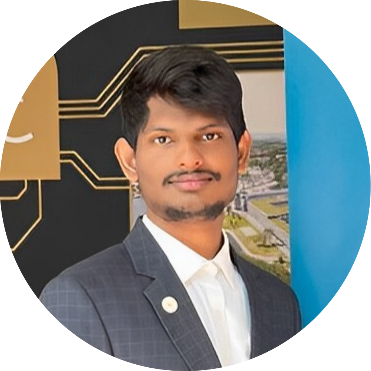
\includegraphics[width=2.7cm,clip]{images/resume_pic_m.png}}
}
\parbox{\dimexpr\linewidth-3.8cm\relax}{
\vspace{-20pt}
\begin{tabularx}{\linewidth}{L r} \\
    {\Huge \scshape  Venkata Sai Yakkshit Reddy Asodi}~
    \href{https://www.cedzlabs.com/yakkshit}{\vspace{1pt}}\\
      Berlin, Germany. \\ \vspace{1pt}
     \small \raisebox{-0.1\height}\faPhone\ +91 8179936156 ~ \href{mailto:saiyakkshit2001@gmail.com}{\raisebox{-0.2\height}\faEnvelope\  {saiyakkshit2001@gmail.com}} ~ 
    \href{https://linkedin.com/in/yakkshit/}{\raisebox{-0.2\height}\faLinkedin\ {yakkshit}}  ~
    \href{https://yakkshit.com/}{\raisebox{-0.2\height}\faGlobe\ {yakkshit.com}}  ~
    \href{https://github.com/yakkshit}{\raisebox{-0.2\height}\faGithub{ yakkshit}}
    \vspace{-8pt}
\end{tabularx}
}
\end{center}

\vspace{-23pt}
%-----------SUMMARY-----------
\section{Summary \faLink}
Passionate Frontend Engineer with 2+ years of experience in developing responsive B2B SaaS applications. Specialized in creating intuitive user interfaces using React and TypeScript, with a strong focus on sustainable technology solutions. Demonstrated ability to take ownership of features and collaborate effectively with product teams to deliver exceptional user experiences. Deeply interested in renewable energy technology and its potential to create positive environmental impact.

%-----------TECHNICAL SKILLS-----------
\section{\href{https://www.linkedin.com/in/yakkshit/details/skills/}{Technical Skills} \faLink}
\begin{itemize}[leftmargin=0.15in, label={}]
\small{\item{
\textbf{Frontend - }{React, TypeScript, Tailwind CSS, HTML5, CSS3, Vue.js} \\
\textbf{Development - }{JavaScript (ES6+), Git, RESTful APIs, Component Libraries} \\
\textbf{Tools - }{Figma, Sketch, Agile/Scrum, Jest, React Testing Library} \\
\textbf{Cloud \& Deployment - }{AWS, Azure, Docker}\\
}}
\end{itemize}
\vspace{-10pt}

%-----------EXPERIENCE-----------
\section{Experience \faLinkedin}
\resumeSubHeadingListStart

\resumeSubheading
{\large Circleup AG \faBuilding}{December 2023 -- July 2024}
{Lead Frontend Engineer}{\faMapMarker \hspace{0.1cm} Zurich, Switzerland}\\
\vspace{10pt}
\textbf{Responsibilities:}
\resumeItemListStart
\vspace{-10pt}
\resumeItem{Led the development of a B2B SaaS platform using React and TypeScript, creating reusable component libraries that improved development efficiency by 40\%. Implemented responsive designs using Tailwind CSS for optimal user experience across devices.}
\resumeItem{Collaborated with product and design teams to implement user-centric features, resulting in a 35\% increase in user engagement. Mentored junior developers and established frontend development best practices.}
\resumeItemListEnd
\vspace{-3pt}
\textbf{Environment:}\emph{React, TypeScript, Tailwind CSS, Git, Agile methodologies}

\resumeSubheading
{Cedzlabs \faBuilding}{March 2023 -- July 2024}
{Frontend Developer}{\faMapMarker \hspace{0.1cm} India}\\
\vspace{10pt}
\textbf{Responsibilities:}
\resumeItemListStart
\resumeItem{Developed and maintained feature-rich frontend applications for B2B clients using React and TypeScript. Implemented responsive UI components and established a comprehensive design system that reduced development time by 25\%.}
\resumeItemListEnd
\vspace{-3pt}
\textbf{Environment:}\emph{React, TypeScript, Tailwind CSS, Git, Jest}

%-----------PROJECTS-----------
\section{Projects \faGithub}
\resumeSubHeadingListStart

\resumeProjectHeading
{\textbf{\href{https://github.com/yakkshit/solar-calculator}{SolarTech Calculator}} $|$ \emph{React, TypeScript, Tailwind CSS}}{January 2024}\\
\vspace{6pt}
\textbf{Description:}
\resumeItemListStart
\resumeItem{Developed an open-source solar panel efficiency calculator that helps users optimize their solar installations. Created an intuitive interface using React and Tailwind CSS, incorporating real-time weather data and energy consumption patterns to provide accurate recommendations.}
\resumeItemListEnd
\vspace{4pt}
\textbf{Tools:}\emph{React, TypeScript, Tailwind CSS, Weather API Integration}

\resumeProjectHeading
{\href{https://github.com/yakkshit/eco-smart}{\textbf{EcoSmart Dashboard}} $|$ \emph{React, TypeScript}}{November 2023}\\
\vspace{6pt}
\textbf{Description:}
\resumeItemListStart
\resumeItem{Built a comprehensive dashboard for monitoring renewable energy systems, featuring real-time data visualization and predictive analytics. Implemented responsive design patterns and optimized performance for large datasets.}
\resumeItemListEnd
\vspace{4pt}
\textbf{Tools:}\emph{React, TypeScript, D3.js, REST APIs}

%-----------ACHIEVEMENTS---------------
\section{Achievements / Contributions}
\resumeSubHeadingListStart
\resumeItemListStart
\resumeItem{Contributed to open-source projects focused on renewable energy monitoring and optimization.}
\resumeItem{Led a team of 3 developers in creating a proof-of-concept for solar panel monitoring system.}
\resumeItem{Actively participate in sustainability-focused tech meetups and renewable energy workshops.}
\resumeItemListEnd

\resumeSubHeadingListEnd
\textbf{Strengths: }\emph{Product-minded, self-starter, attention to detail, passionate about renewable energy} \\
\textbf{Languages: }\emph{Telugu - Native $|$ English - Fluent $|$ Hindi - Fluent $|$ German - Elementary $|$ Swedish - Elementary}

\vspace{10pt}
\end{document}